\documentclass[usenatbib]{article}
\usepackage{url,times,graphicx,amsmath,amsfonts,amssymb,color,epsfig,varioref,subfigure,comment,natbib}
\usepackage{color}

\title{{\it N}-body simulations with Jordan-Brans-Dicke}
\author{Hans Winther}

\begin{document}
\maketitle

\subsection*{Introduction}

The {\it N}-body equations are quite simple once we use some approximations. Note that there is no problem not performing these approximation (apart from the quasi-static one) if desirable. The full equation set for a very similar model has been derived before, see e.g. Li et al. [1] - the JBD model corresponds to taking $f(\varphi) = \frac{\kappa^2\varphi^2}{4\omega} - 1$ and redefining $\frac{\kappa^2\varphi^2}{4\omega} \to \varphi$. Below I will give the equations in their simplest form with all approximations included. Using same notation as in Lima \& Ferreira [2] and Avilez \& Skordis [3]\footnote{References: \newline [1]: https://arxiv.org/pdf/1009.1400.pdf \newline [2]: https://arxiv.org/pdf/1506.07771.pdf \newline [3]: https://arxiv.org/pdf/1303.4330.pdf }.

\subsection*{Approximations}

The main approximations used is that perturbations of $\phi$ will always be small. Splitting $\phi = \overline{\phi} + \delta\phi$ then in the quasi-static approximation we have
$$\frac{1}{a^2}\nabla\delta\phi \simeq \frac{\kappa^2}{2(3+2\omega)}\delta\rho_m$$
so $\delta\phi \simeq \frac{1}{\phi(3+2\omega)}\Phi_N$ where $\Phi_N$ is the standard Newtonian gravitational potential in GR. In a cosmological simulation we have $\Phi_N \lesssim 10^{-5}$ and also since $\omega\gtrsim 100$ this means we can neglect terms $\phi_{,\mu}\phi_{,\nu}$ relative to $\rho_m$ in the Einstein equation.

\subsection*{{\it N}-body equations}

The $00$-component of the Einstein equation
$$G_{\mu\nu} = \frac{\kappa^2}{\phi}T_{\mu\nu} + \frac{\omega}{\phi^2}(\phi_{,\mu}\phi_{,\nu} - \frac{1}{2}g_{\mu\nu}(\partial\phi)^2) + \frac{1}{\phi}(\phi_{,\nu;\mu} - g_{\mu\nu}\square\phi) - \frac{\kappa^2\Lambda}{\phi}$$
gives us the Poisson equation
$$\nabla^2\Phi \simeq \frac{\kappa^2}{2} a^2\delta\rho_m \cdot \frac{1}{\overline{\phi}}\frac{4+2\omega}{3+2\omega}$$
The {\it N}-body (geodesic) equation becomes
$$\ddot{x} + 2H\dot{x} = -\frac{1}{a^2}\nabla\Phi$$
Thus the main modification is the presence of an effective (time-dependent) gravitational constant instead of $G$ in the Poisson equation
$$\frac{G_{\rm eff}}{G} = \frac{1}{\overline{\phi}}\frac{4+2\omega}{3+2\omega}$$
The field should be normalized such that $\frac{\kappa^2}{\overline{\phi}_0}\frac{4+2\omega}{3+2\omega} = 8\pi G_N$. If $\kappa^2 = 8\pi G_N$ then we simply take $\overline{\phi}_0 \equiv \frac{4+2\omega}{3+2\omega}$.

\subsection*{Background cosmology and evolution of $\phi$}

The background cosmology and $\phi$ is determined by
$$E^2(a)\left(1 + \frac{d\log \overline{\phi}}{d\log a} - \frac{\omega}{6}\left(\frac{d\log \overline{\phi}}{d\log a}\right)^2\right) = \frac{\phi_0}{\overline{\phi}}\left[\frac{\Omega_{m0}}{a^3} + \frac{\Omega_{r0}}{a^4} + \Omega_{\Lambda 0}\right]$$
$$E(a)\frac{d}{d\log a}\left[E(a)a^3 \frac{d\log \overline{\phi}}{d\log a} \frac{\overline{\phi}}{\phi_0}\right] = \frac{3 a^3}{3+2\omega}\left[\frac{\Omega_{m0}}{a^3} + 4 \Omega_{\Lambda 0}\right]$$
where $\Omega_{\Lambda 0} = 1 + \frac{d\log \phi_0}{d\log a} - \frac{\omega}{6}\left(\frac{d\log \phi_0}{d\log a}\right)^2 - \Omega_{m0} - \Omega_{r0}$ and $\phi_0 = \frac{4+2\omega}{3+2\omega}$. We solve these by starting the integration deep inside in the radiation era with the initial conditions $\phi_i$ and $\frac{d\log \phi_i}{d\log a} = 0$ and tune the value of $\phi_i$ such that $\phi(a=1) = \phi_0$ (this is what Avilez \& Skordis called restricted Brans-Dicke models). The value of $\frac{d\log \phi_0}{d\log a}$ needed to determine $\Omega_{\Lambda 0}$ is set to $\frac{1}{1+\omega}$ and corrected at every step until we have convergence (the true value is roughly $\simeq (1.9 - 1.1\Omega_{m0})/(1+\omega)$ for realistic values of $\Omega_{m0}$). See the plots below for the results when $\omega = 50$. The results I find gives a reasonable match the Fig. 1 in Lima \& Ferreira (though $\phi(a=1) = \phi_0$ is not imposed there).

\begin{figure}
\begin{center}
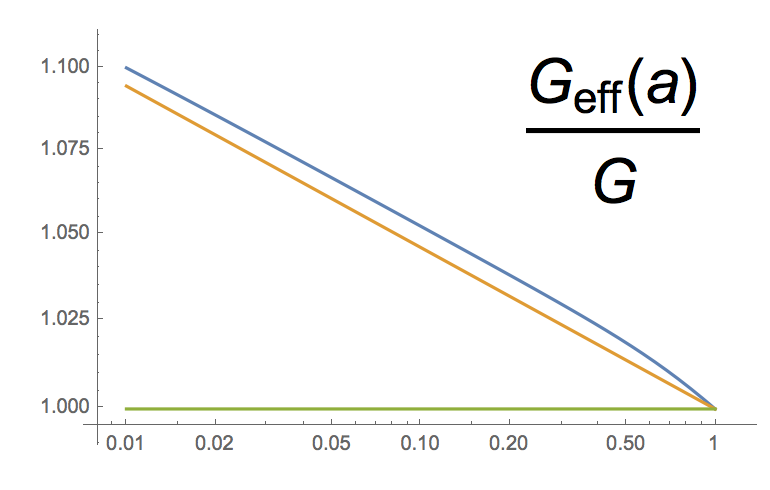
\includegraphics[width=0.9\columnwidth]{plots/pp1.png}
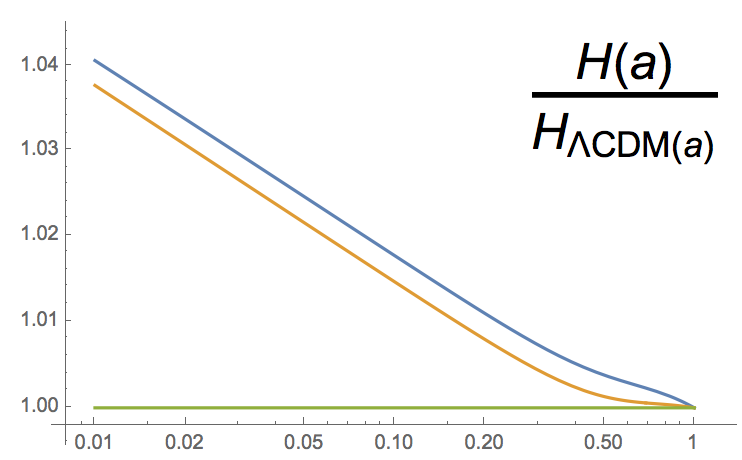
\includegraphics[width=0.9\columnwidth]{plots/pp2.png}
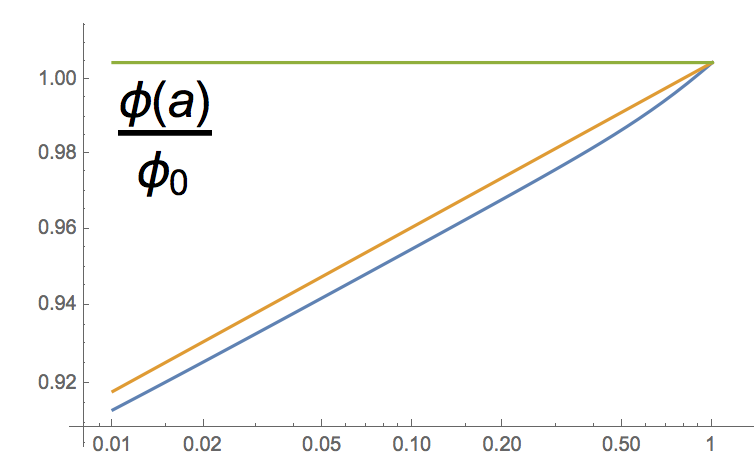
\includegraphics[width=0.9\columnwidth]{plots/pp3.png}
\caption{The evolution of $\phi(a)$, $H(a)/H_{\Lambda CDM}(a)$ and $\frac{G_{\rm eff}(a)}{G}$ for $\omega = 50$, $\Omega_{m0} = 0.3$ and $\Omega_{r0} = 8.4\cdot 10^{-5}$. The orange lines shown the results of using the approximation $\phi(a) = \phi_0 a^{\frac{1}{1+\omega}}$ and the blue lines are the full numerical solution. The error of using this approximation is $\sim 0.5\%$ for $\omega = 50$ and drops to $0.05\%$ for $\omega = 500$.}
\end{center}
\end{figure}

\subsection*{Initial conditions}

The IC are generated using second order lagrangian perturbation theory. We need a $P(k)$ or $T(k)$ from CAMB or similar at $z=0$. This is then scaled backwards to the initial redshift using the (1LPT) growth-factor which is determined by
$$\ddot{D} + 2H\dot{D} = \frac{3}{2}\frac{\Omega_{m0}}{a^3 H^2}\frac{\phi_0}{\overline{\phi}} D$$
For 2LPT it should be enough to simply use the EdS approximation $D_2 = -\frac{3}{7}D_1^2$.

\subsection*{Summary}

The equation we solve in the {\it N}-body:
$$\ddot{x} + 2H\dot{x} = -\frac{1}{a^2}\frac{\phi_0}{\overline{\phi}}\nabla \Phi_N,~~~~~\nabla^2\Phi_N = \frac{3}{2}\Omega_{m0}H_0^2 a^{-1} \delta_m$$
where the background is determined by:
$$E^2(a)\left(1 + \frac{d\log \overline{\phi}}{d\log a} - \frac{\omega}{6}\left(\frac{d\log \overline{\phi}}{d\log a}\right)^2\right) = \frac{\phi_0}{\overline{\phi}}\left[\frac{\Omega_{m0}}{a^3} + \Omega_{\Lambda 0}\right]$$
$$E(a)\frac{d}{d\log a}\left[E(a)a^3 \frac{d\log \overline{\phi}}{d\log a} \frac{\overline{\phi}}{\phi_0}\right] = \frac{3 a^3}{3+2\omega}\left[\frac{\Omega_{m0}}{a^3} + 4 \Omega_{\Lambda 0}\right]$$
and these are solved with initial conditions set in the deep radiation era with $\frac{d\log\phi}{d\log a} = 0$ and $\phi_i$ tuned as to give $\phi(a=1) = \phi_0$ implying $\frac{G_{\rm eff}}{G} = 1$ at the present time.

\end{document}

\subsection*{Alternative way}

An alternative way is to first transform the equations to the Einstein-frame and solve it there (and the transform back after solving). With a conformal transformation $g_{\mu\nu}\to g_{\mu\nu} A^2(\phi)g_{\mu\nu}$ where $A(\phi) = e^{\frac{\beta\phi}{M_{\rm Pl}}}$ with $2\beta^2 = \frac{1}{3+2\omega_{\rm BD})}$ then JBD action transforms into
\begin{align}
\int\sqrt{-\hat{g}}{\rm d}^4x\left[\varphi \hat{R} - \frac{\omega_{\rm BD}}{\varphi}(\hat{\nabla}\varphi)^2 \right] + S_m(\hat{g}_{\mu\nu};\psi_m) \\
\to \int\sqrt{-g}{\rm d}x^4\left[\frac{R}{8\pi G} - \frac{1}{2}(\nabla\phi)^2\right] + S_m(g_{\mu\nu}A^2(\phi);\psi_m)
\end{align}
This is exactly the same form as we have for other {\it N}-body simulations (for chameleons etc.). In this frame particles will have a time-varying mass giving rise to an additional $\dot{x} \frac{\beta\dot{\phi}}{M_{\rm Pl}}$ friction-term in the geodesic equation. It's easier to just solve everything in the matter (Jordan) frame.




The $R_{00} - \overline{R}_{00}$ component of the Einstein equation gives us the Poisson equation
$$\nabla^2\Phi = \frac{\kappa^2}{2}a^2\left[\frac{\rho_m}{\varphi} - \frac{\overline{\rho}_m}{\overline{\varphi}}\right]\cdot \frac{4+2\omega}{3+2\omega}$$
Letting the EM tensor be that of dark matter particles $T^m_{\mu\nu}(r) = \sum \frac{2}{\sqrt{-g}}\dot{x}_\mu\dot{x}_\nu \delta(r - x)$ then conservation of this, $\nabla^\mu T^m_{\mu\nu} = 0$, gives us the geodesic equation
$$\ddot{x} + 2H\dot{x} = - \frac{1}{a^2}\nabla\Phi$$
In this form the only modification is in the effective Newton's constant
$$\frac{G_{\rm eff}}{G} = \frac{1}{\varphi}\frac{4+2\omega}{3+2\omega}$$
The field $\varphi$ is found from
$$\ddot{\overline{\varphi}} + 3H\dot{\overline{\varphi}} = \frac{\overline{\rho_m}\kappa^2}{3+2\omega}$$
Since the perturbations in $\varphi$ will be small ($\sim \Phi \lessim 10^{-5}$ is a cosmological simulation) we can take $\varphi \approx \overline{\varphi}$.

Another approach is to go to the Einstein-frame. With a conformal transformation $g_{\mu\nu}\to g_{\mu\nu} A^2(\phi)g_{\mu\nu}$ where $A(\phi) = e^{\frac{\beta\phi}{M_{\rm Pl}}}$ with $2\beta^2 = \frac{1}{3+2\omega_{\rm BD})}$ then JBD action transforms into
$$\int\sqrt{-\hat{g}}{\rm d}^4x\left[\varphi \hat{R} - \frac{\omega_{\rm BD}}{\varphi}(\hat{\nabla}\varphi)^2 \right] + S_m(\hat{g}_{\mu\nu};\psi_m) \to \int\sqrt{-g}{\rm d}x^4\left[\frac{R}{8\pi G} - \frac{1}{2}(\nabla\phi)^2\right] + S_m(g_{\mu\nu}A^2(\phi);\psi_m)$$
In this frame particles will have a time-varying mass giving rise to an additional $\dot{x} \frac{\beta\dot{\phi}}{M_{\rm Pl}}$ friction-term in the geodesic equation.
\end{document}

The Einstein equation can now be written
$$G_{\mu\nu} = A(\phi)T^m_{\mu\nu} + T^\phi_{\mu\nu}$$
This way of writing it ensures that $T^m$ is conserved under the cosmological evolution, i.e. $T^m \propto a^{-3}$.


\section*{-body Equations}
Going to the Einstein-frame with a conformal transformation $g_{\mu\nu}\to g_{\mu\nu} A^2(\phi)g_{\mu\nu}$ where $A(\phi) = e^{\frac{\beta\phi}{M_{\rm Pl}}}$ with $2\beta^2 = \frac{1}{3+2\omega_{\rm BD})}$ then JBD action transforms into
$$\int\sqrt{-\hat{g}}{\rm d}^4x\left[\varphi \hat{R} - \frac{\omega_{\rm BD}}{\varphi}(\hat{\nabla}\varphi)^2 \right] + S_m(\hat{g}_{\mu\nu};\psi_m) \to \int\sqrt{-g}{\rm d}x^4\left[\frac{R}{8\pi G} - \frac{1}{2}(\nabla\phi)^2\right] + S_m(g_{\mu\nu}A(\phi);\psi_m)$$
The Einstein equation can now be written
$$G_{\mu\nu} = A(\phi)T^m_{\mu\nu} + T^\phi_{\mu\nu}$$
where $T^m_{\mu\nu}$ as defined is co-variantly conserved, i.e. $\frac{d}{dt}(\overline{\rho}_ma^3) = 0$ in the cosmological context (the conserved matter density in the Jordan-frame is likewise $\frac{\rho_m}{\varphi}$). The scalar-field $\phi$ can be decomposed as $\phi = \overline{\phi}(a) + \delta\phi(x,t)$. At the background level we have
$$\ddot{\overline{\phi}} + 3H\dot{\overline{\phi}}(a) + \frac{\beta}{M_{\rm Pl}}A(\overline{\phi})\overline{\rho}_m = 0$$
and in the quasi-static limit we find
$$\frac{1}{a^2}\nabla^2\delta\phi = \frac{\beta}{M_{\rm Pl}}[A(\phi)\rho_m - A(\overline{\phi})\overline{\rho}_m]$$
The standard Poisson equation reads (neglecting small terms)
$$\frac{1}{a^2}\nabla^2\Phi = \frac{3}{2}\Omega_m [A(\phi)\rho_m - A(\overline{\phi})\overline{\rho}_m]$$
With the approximation $|\overline{\phi}| \gg |\delta\phi|$ (the former is $\sim 1$ and the latter is $\sim \Phi_N \lesssim 10^{-5}$) we get
$$\frac{1}{a^2}\nabla^2\Phi \simeq \frac{3}{2}\Omega_m A(\overline{\phi})\overline{\rho}_m \delta_m$$
and
$$\delta\phi \simeq 2\beta^2 M_{\rm Pl}\Phi$$
The N-body equations are now
$$\ddot{x} + 2H\left(1 + \frac{1}{2}\frac{d\log A(\phi)}{d\log a}\right)\dot{x} = -\frac{1}{a^2}\nabla\Phi - \frac{\beta}{a^2}\frac{\nabla\phi}{M_{\rm Pl}}$$
which can be written
$$\ddot{x} + 2H\left(1 + \frac{1}{2}\frac{d\log A(\phi)}{d\log a}\right)\dot{x} = -\frac{1}{a^2}\nabla\Phi_{\rm eff}$$
where
$$\nabla^2\Phi_{\rm eff} = \frac{3}{2}\Omega_m a^2 \overline{\rho}_m \delta_m \cdot \frac{G_{\rm eff}}{G}$$
and
$$\frac{G_{\rm eff}}{G} = A(\overline{\phi})(1+2\beta^2) = A(\overline{\phi})\frac{4+2\omega_{\rm BD}}{3+2\omega_{\rm BD}}$$
There are two main modifications above: 1) a friction term coming from the fact that particles have a time-dependent mass in the Einstein-frame and 2) a modified Poisson equation due to an effective Newtonian constant. Both of these effects are easy to include in an N-body code.

If we want a $\Lambda$CDM cosmology in the Jordan-frame then we convert this to the EF using
$$a_{\rm JF} = a_{\rm EF} A(\phi)$$

\end{document}

The time-dependent factor is
$$\frac{d\log A}{d\log a} = \frac{\beta d\phi}{dt} = -\frac{\dot{\Phi}_{\rm BD}}{\Phi_{\rm BD}}$$

The time-evolution of $\Phi_{\rm BD}$, since we are assuming a $\Lambda$CDM cosmology, is given by
$$\ddot{\phi} + 3H\dot{\phi} + \frac{\beta\dot{\phi}}{M_{\rm Pl}}A(\phi)\overline{\rho}_m = 0$$
\end{document}

For a single DM particle the effective EM tensor entering the Einstein equations is
$$T^{\mu\nu}(r) = \frac{1}{\phi}\frac{2m_0\dot{x}^\mu \dot{x}^\nu \delta(r - x)}{\sqrt{-g}}$$
Taking the divergence and using that $\nabla^\mu T_{\mu\nu} = 0$ we get the geodesic equation
$$\ddot{x} + 2H\dot{x} - \frac{\dot{\phi}}{\phi}\dot{x} = - \frac{1}{a^2}\left[\nabla\Phi - \frac{\nabla\phi}{\phi}\right]$$
where
$$\nabla^2\Phi = \frac{3}{2\phi}\Omega_m a^2 H_0^2\delta\rho_m$$
Splitting $\phi(x,a) = \phi(a) + \delta\phi$ and using the quasi-static approximation we get
$$\nabla^2\delta\phi = - \frac{2}{3+2\omega}\cdot \frac{3}{2}\Omega_m a^2 H_0^2\delta\rho_m \implies \frac{\delta\phi}{\phi(a)} = - \frac{2}{3+2\omega}\Phi$$
and we can write the system above as
$$\ddot{x} + 2H\left[1 - \frac{1}{2}\frac{d\log \phi}{d\log a}\right]\dot{x} = - \frac{1}{a^2}\nabla\Phi_{\rm eff}$$
where
$$\nabla^2\Phi_{\rm eff} = \frac{3}{2}\frac{G_{\rm eff}(a)}{G}\Omega_m a^2 H_0^2\delta\rho_m$$
is the effective gravitational potential and
$$\frac{G_{\rm eff}(a)}{G} = \frac{1}{\phi(a)} \frac{4+2\omega}{3+2\omega}$$
There are two main modifications here
\begin{itemize}
\item The addition of a time-dependent Newton's constant
\item The addition of a friction term (due to time-variation of particle masses relative to the evolving Planck scale: $m(\phi) = \frac{m_0}{\phi}$).
\end{itemize}

\end{document}

Start in the Jordan-frame. Write down the N-body equations.

$$\ddot{x} + 2H\dot{x} = $$

The N-body equations can be written
$$\ddot{x} + 2H\dot{x} + \frac{d\log m(\phi)}{dt}\dot{x} = - \frac{1}{a^2}\frac{G_{\rm eff}(a)}{G}\nabla\Phi$$
where $m(\phi)$ is the mass of the dark matter particles as function of time (since the Planck mass varies).

This term is given by
$$ 2H\dot{x} + \frac{d\log m(\phi)}{dt}\dot{x} \sim eq \left(2  - \frac{1}{1+\omega_{\rm BD}}\right)H\dot{x}$$
which will be small.

\end{document}

We first go to the Einstein frame by a conformal transformation and redefine $\phi = e^{-2\frac{\beta\sigma}{M_{\rm Pl}}}$ where $\beta = \frac{1}{\sqrt{2}\sqrt{3+2\omega_{\rm BD}}}$. This leads to an action with a canonical scalar coupled conformally via $g_{\mu\nu}e^{\frac{2\beta\sigma}{M_{\rm Pl}}}$ to matter. The background scalar field equation becomes
$$\ddot{\overline{\sigma}} + 2H\dot{\overline{\sigma}}  + \frac{\beta\overline{\rho}_m}{M_{\rm Pl}} = 0$$
For perturbations we set $\sigma = \overline{\sigma} + \delta\sigma$ and in the quasi-static limit this gives
$$\nabla^2\delta\sigma = \frac{\beta a^2}{M_{\rm Pl}}\delta\rho_m$$
so $\delta\sigma = 2\beta M_{\rm Pl} \Phi_N$ where $\Phi_N$ is the gravitational potential
$$\nabla^2\Phi = \frac{3}{2}\Omega_m a H_0^2\delta_m$$
The N-body equations then becomes
$$\ddot{x} + 2H\dot{x} = -\frac{1}{a^4}(1+2\beta^2)\nabla\Phi$$
$$\Delta^2\Phi = \frac{3}{2}a\Omega_m \cdot \frac{G_{\rm eff}(a)}{G} \cdot \delta$$
where
$$\frac{G_{\rm eff}(a)}{G} = \frac{1}{\phi(a)} \frac{4+2\omega_{\rm BD}}{3+2\omega_{\rm BD}}$$
with
$$\phi(a) = \frac{3+2\omega_{\rm BD}}{4+2\omega_{\rm BD}}a^{\frac{1}{1+\omega_{\rm BD}}}$$
This assumes the attractor solution in the matter dominated era. In general we have
$$\ddot{\phi} + 3H\dot{\phi} = \frac{\kappa^2\rho_m}{3+2\omega_{\rm BD}}$$
which we solve using IC such that $\phi = \phi_0$ today.

\end{document}
